\documentclass[tikz,border=10pt]{standalone}
\usepackage{tikz}
\begin{document}
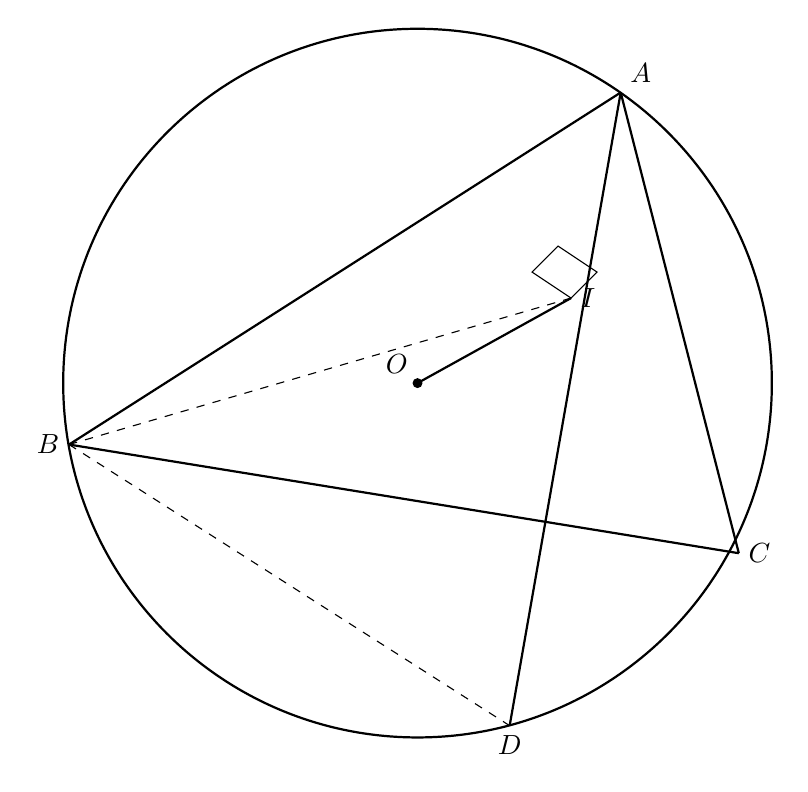
\begin{tikzpicture}[scale=1.5]
\coordinate (O) at (0,0);
\coordinate (A) at (1.72,2.46);
\coordinate (B) at (-2.95,-0.52);
\coordinate (C) at (2.72,-1.44);
\coordinate (D) at (0.78,-2.90);
\coordinate (I) at (1.30,0.72);
\draw[thick] (O) circle (3);
\draw[thick] (B) -- (A);
\draw[thick] (A) -- (C);
\draw[thick] (B) -- (C);
\draw[thick] (A) -- (D);
\draw[thick] (O) -- (I);
\draw[dashed] (B) -- (I);
\draw[dashed] (B) -- (D);
\draw (0.97,0.94) -- (1.19,1.16) -- (1.52,0.94) -- (1.30,0.72) -- cycle;
\fill (O) circle (1.2pt);
\node[above left] at (O) {$O$};
\node[above right] at (A) {$A$};
\node[left] at (B) {$B$};
\node[right] at (C) {$C$};
\node[below] at (D) {$D$};
\node[right] at (I) {$I$};
\end{tikzpicture}
\end{document}
